\documentclass[a4, 13pt]{article}
\usepackage[utf8]{inputenc}
\usepackage{graphicx}
\title{Resume \\ \vspace{0.3cm }\\ Aplikasi Akademik Sederhana\\ Basis Data II}
\author{Okky Yudistira (1184087) \\ Kelas: D4 TI 2A \vspace{0.3cm} }
\date{November 2019}

\begin{document}


\section{Rangkuman / Resume Materi}
Untuk Pembuatan Aplikasi Akademik Sedeherhana Kita harus terlebih dahulu mempunya data data yang
Sudah di Normalisasi , dan Di sini saya mengambil contoh data dari Modul 3 Database 1. Dimana Mempunyai
5 Tabel yang belum Di normalisasi
\begin{figure}[!htbp]
        \centering
        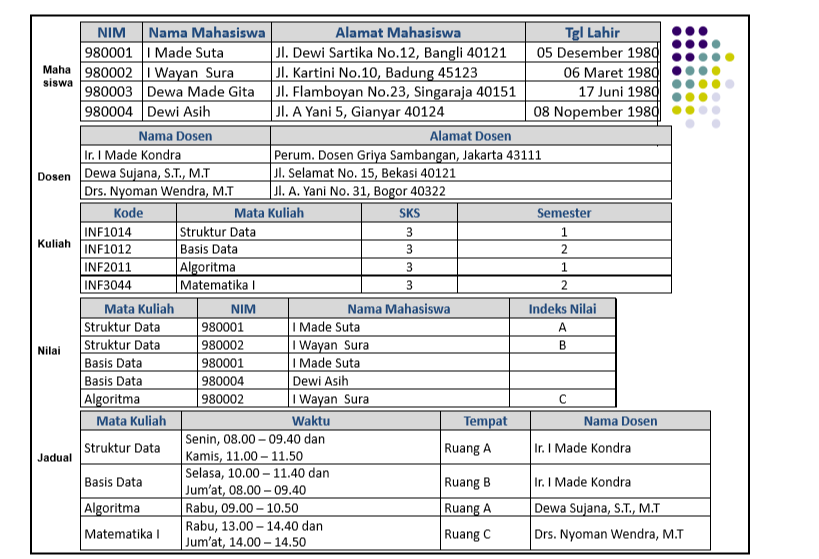
\includegraphics[width=16cm, height=12cm]{pictures/1.png}
        \caption{Contoh Table Yang belum dinormalisasi}
        \label{fig:my_label}
    \end{figure}
    \vspace{2cm}
    
    \section{Membuat Normalisasi Pada Excel}
    Dan Dibawah ini adalah Contoh Foto Data Yang sudah dinormalisasi dalam 5 table dan di masukan Ke dalam Excel
    \begin{figure}[!htbp]
        \centering
        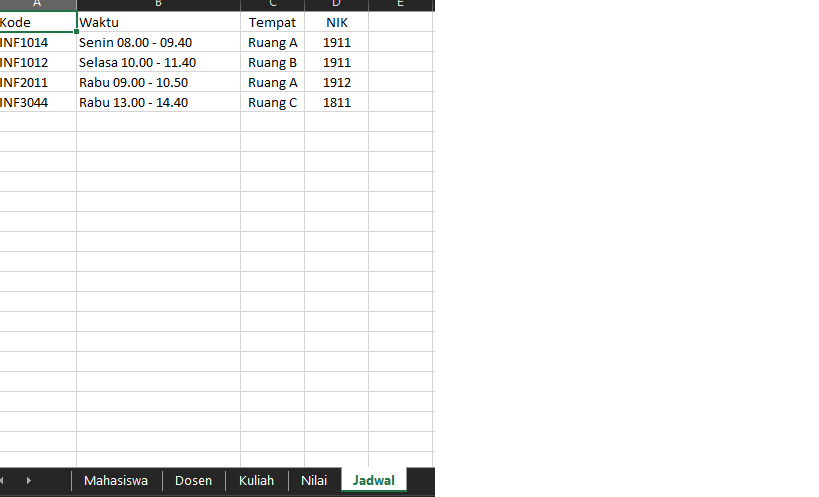
\includegraphics[width=16cm, height=12cm]{pictures/2.png}
        \caption{Contoh Table Yang telah dinormalisasi Dari sheet ke 5 (jadwal)}
        \label{fig:my_label}
    \end{figure}
    \vspace{2cm}
    
    \section{Mulai Mengupload File Ke APEX Online}
    Sebelum Mengupload Amati Dulu Data nya apakah sudah benar benar layak dan Tidak acak acakan agar nanti nya tidak terjadi kesalahan yang bikin kita menjadi kerepotan. Jika sudah Silahkan Login Ke apex Online masing masing lalu Masuk ke App Builder dan Ke menu Websheet aplication Dan Masuk Ke From A File untuk mengupload Data excel
    \begin{figure}[!htbp]
        \centering
        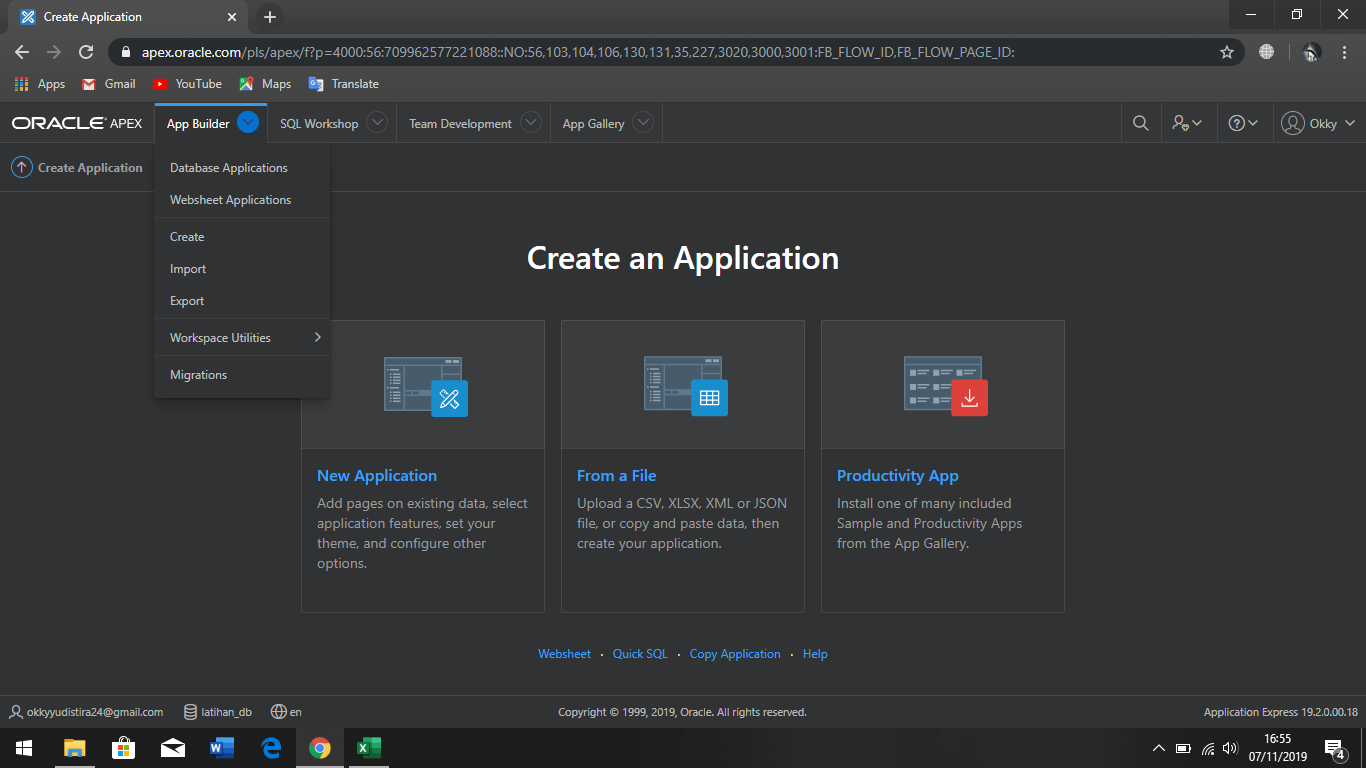
\includegraphics[width=16cm, height=12cm]{pictures/A.png}
        \caption{Contoh Tampilan Awal}
        \label{fig:my_label}
    \end{figure}
    \vspace{2cm}
    
      \section{Load Data }
   Beri Nama Table yang di Inginkan sesuai Data pada Sheet yang ada di excel tdi Dan jangan Lupa konfigurasikan Untuk mengatur data yang sesuai
    \begin{figure}[!htbp]
        \centering
        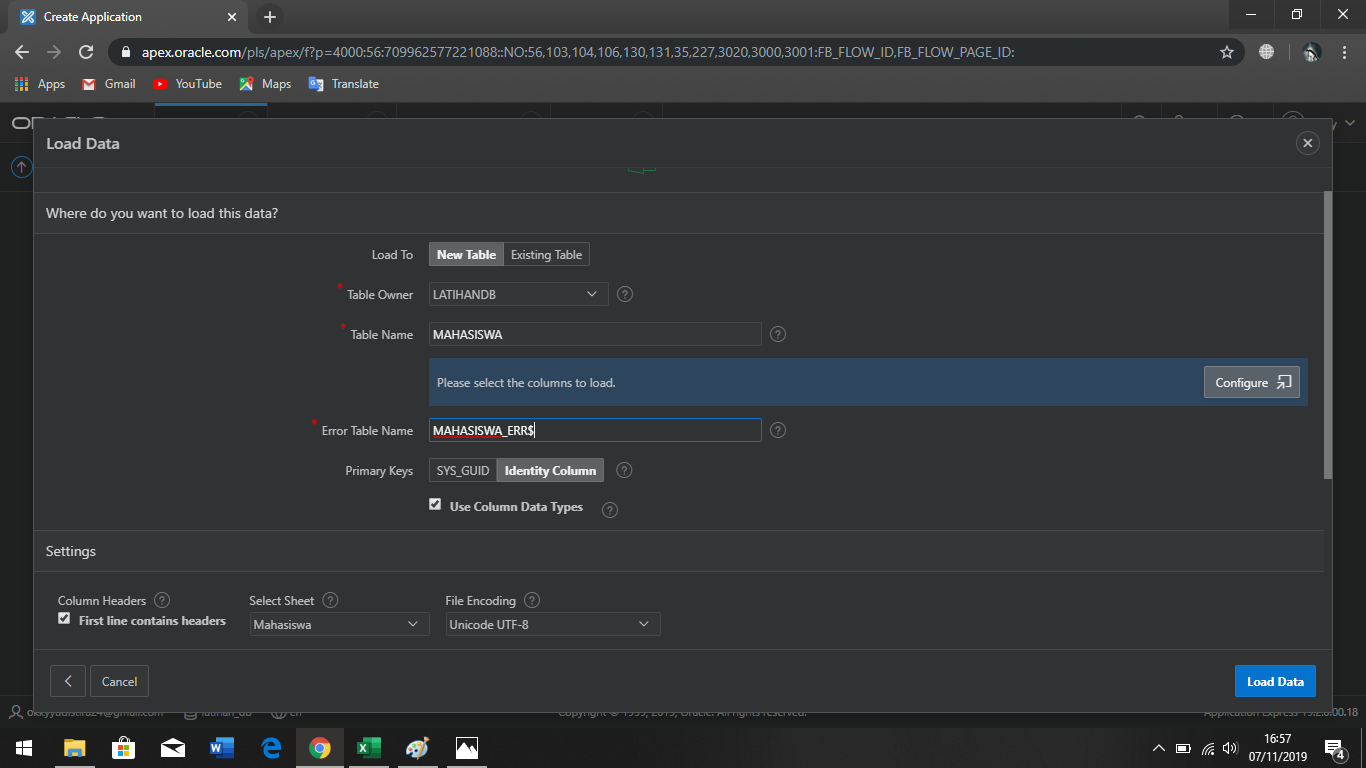
\includegraphics[width=15cm, height=15cm]{pictures/B.png}
        \caption{Contoh Saat pembuataan table mahasiswa}
        \label{fig:my_label}
    \end{figure}
    \vspace{2cm}
    
      \section{konfigurasi}
      pilih sheet yang sesuai agar data yang di load tidak salah. Setelah itu save change 
    \begin{figure}[!htbp]
        \centering
        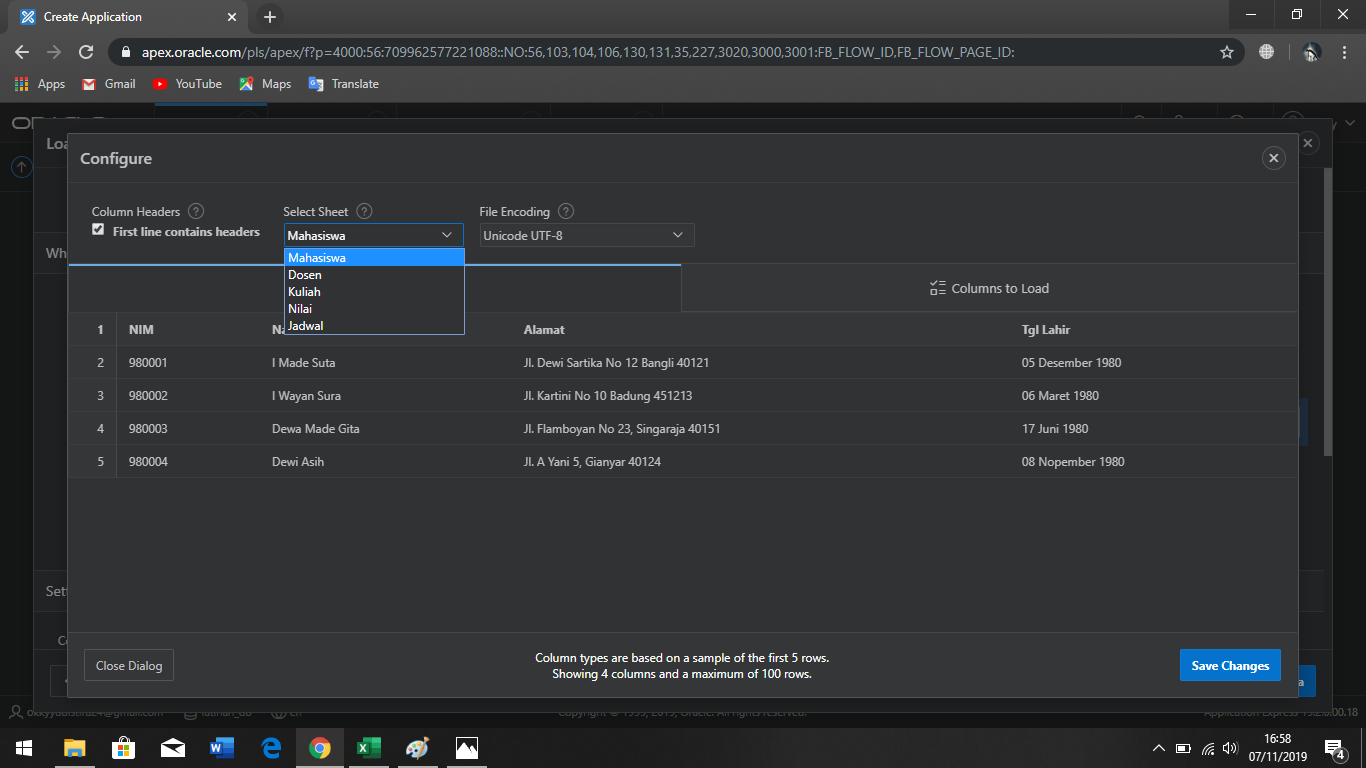
\includegraphics[width=16cm, height=12cm]{pictures/C.png}
        \caption{Contoh Konfigurasi sheet yang diingikan sesuai sheet)}
        \label{fig:my_label}
    \end{figure}
    \vspace{2cm}
    
    
      \section{Preview Data}
     Teliti lagi apakah Datanya sudah benar Di preview terlebih dahulu sebelum di Load. jika sudah benar lalu load
    \begin{figure}[!htbp]
        \centering
        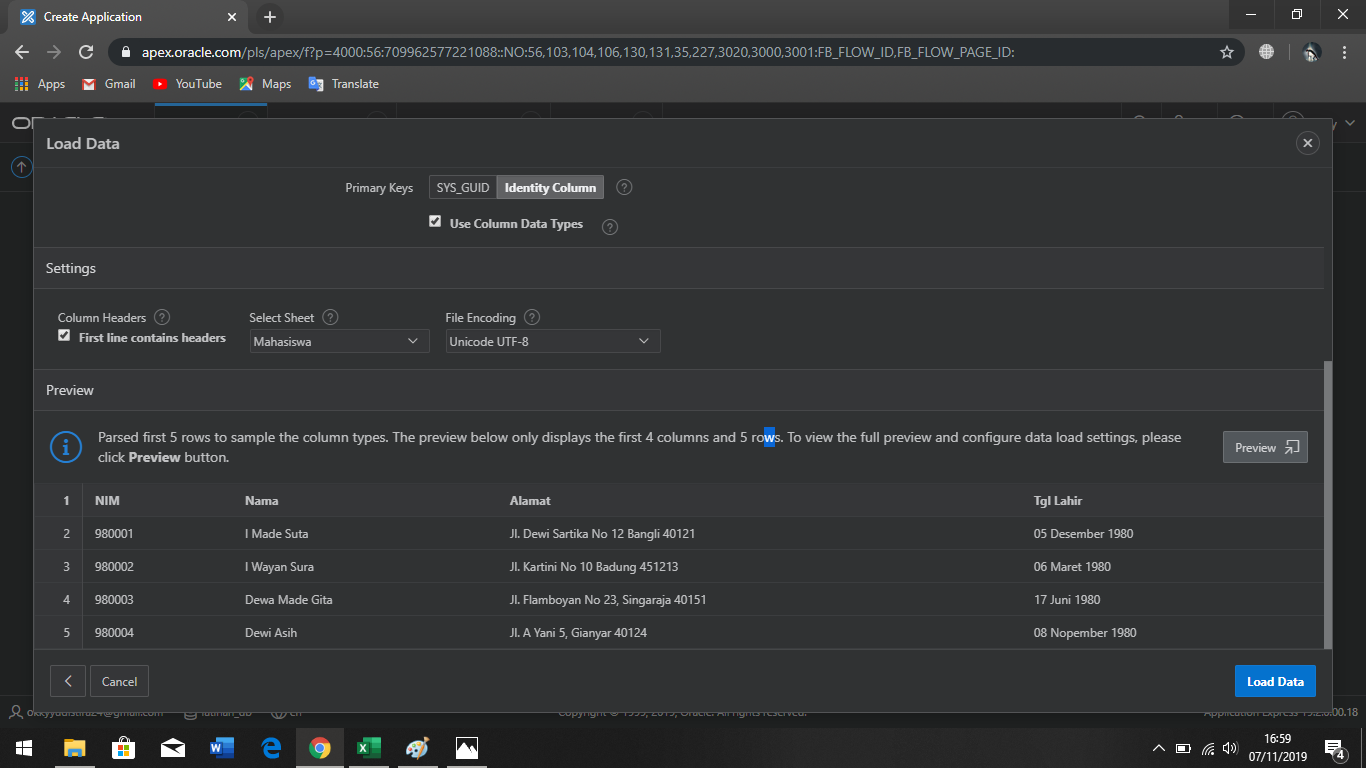
\includegraphics[width=16cm, height=12cm]{pictures/D.png}
        \caption{Preview Data)}
        \label{fig:my_label}
    \end{figure}
    \vspace{2cm}
    
     \section{Constraints}
     Contraints Berfungsi sebagai penentuan primary key , Foregin key dll. Di table mahasiswa ini saya memberikan PK pada NIM
    \begin{figure}[!htbp]
        \centering
        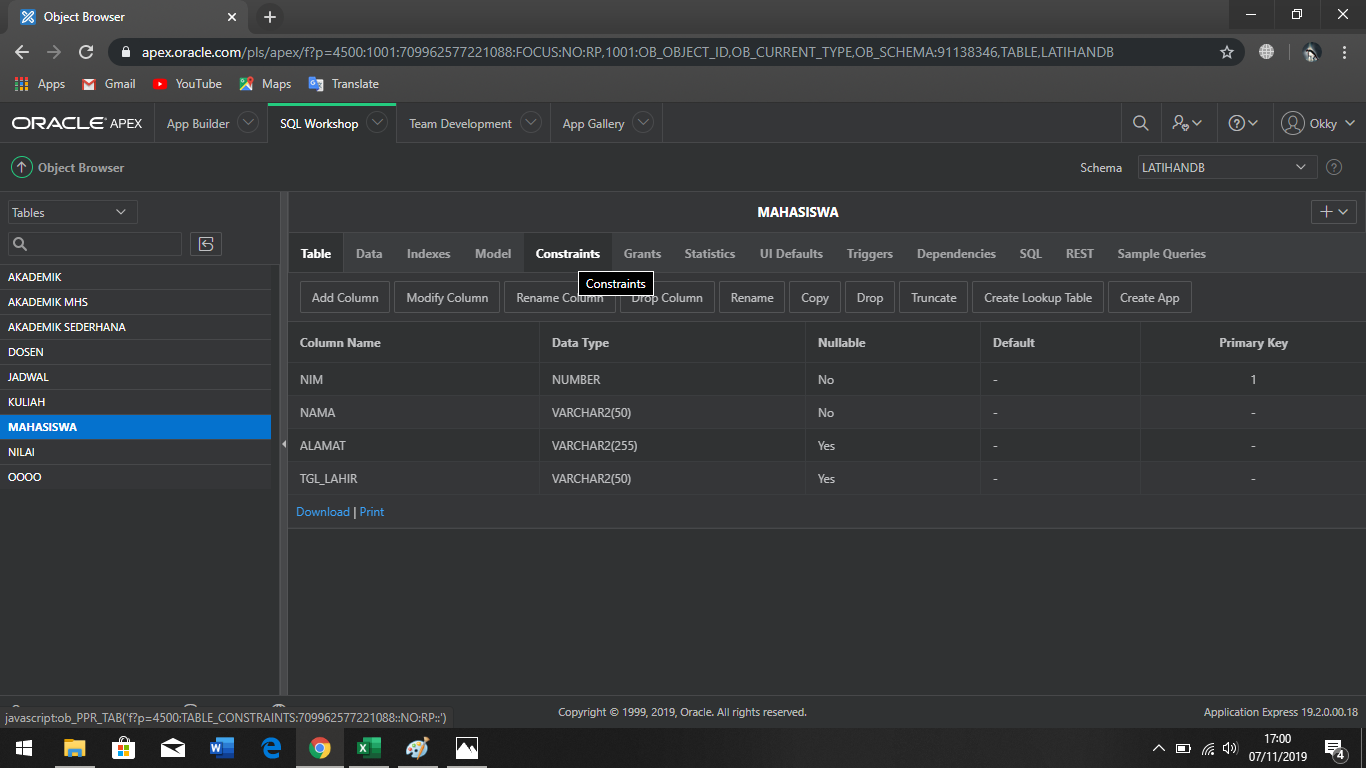
\includegraphics[width=16cm, height=12cm]{pictures/E.png}
        \caption{Contoh Contraints Dan Beberapa table)}
        \label{fig:my_label}
    \end{figure}
     \begin{figure}[!htbp]
        \centering
        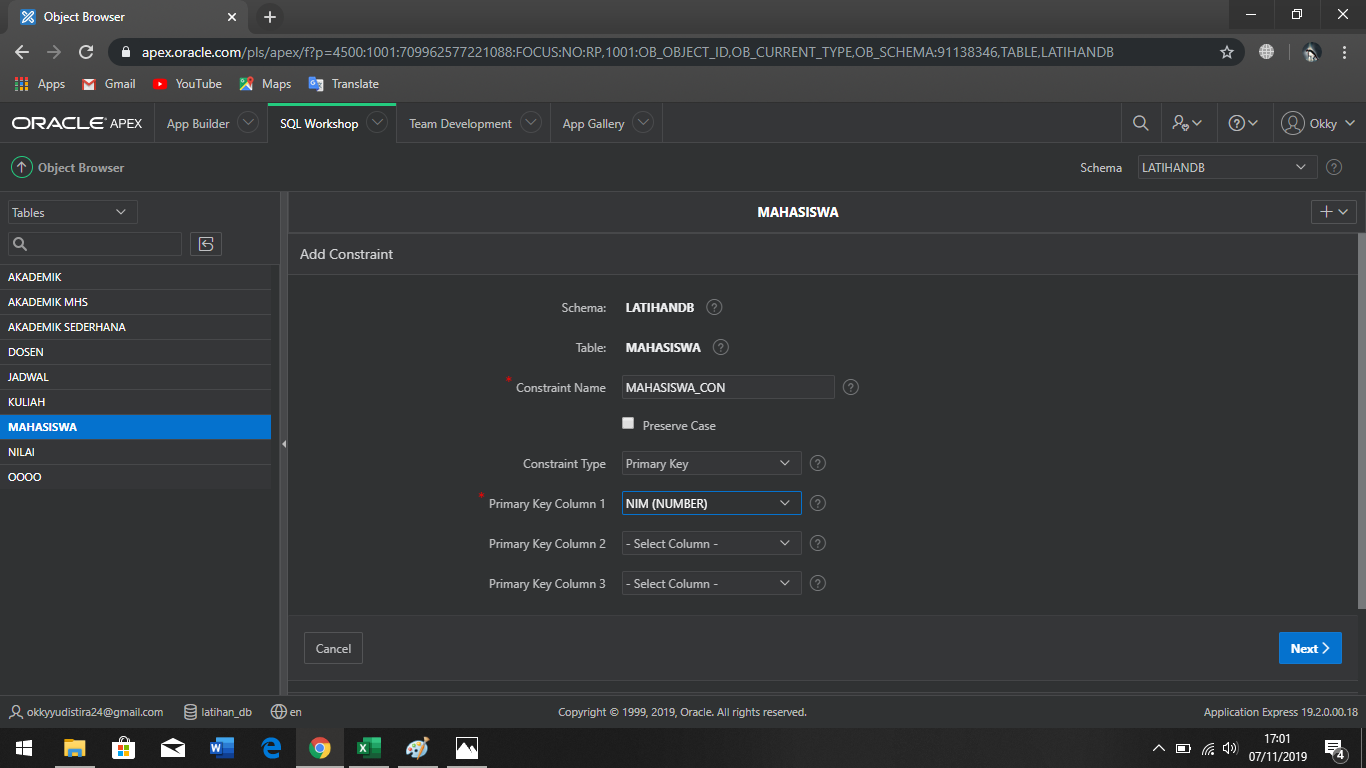
\includegraphics[width=16cm, height=12cm]{pictures/F.png}
        \caption{Contoh Contraints)}
        \label{fig:my_label}
    \end{figure}
     \begin{figure}[!htbp]
        \centering
        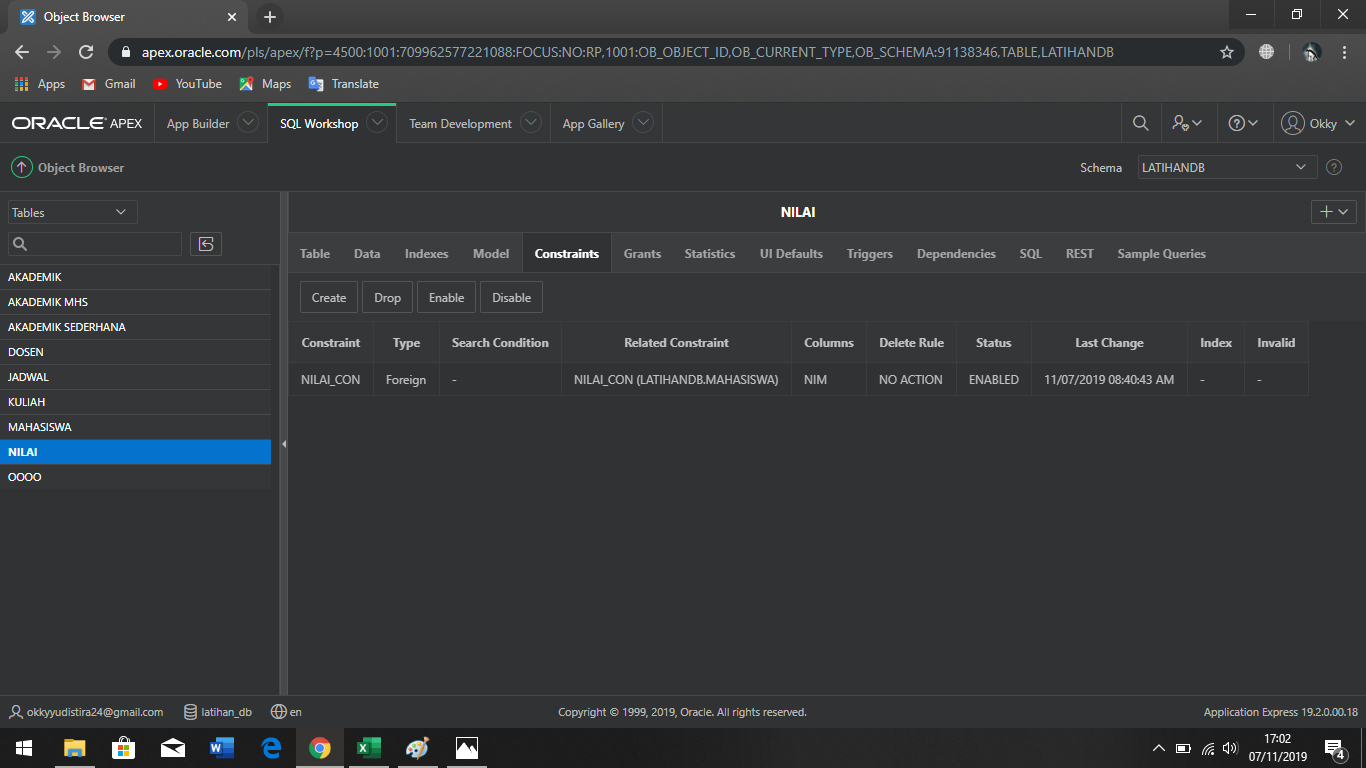
\includegraphics[width=16cm, height=12cm]{pictures/G.png}
        \caption{Contoh Contraints)}
        \label{fig:my_label}
    \end{figure}
    \vspace{2cm}
     \begin{figure}[!htbp]
        \centering
        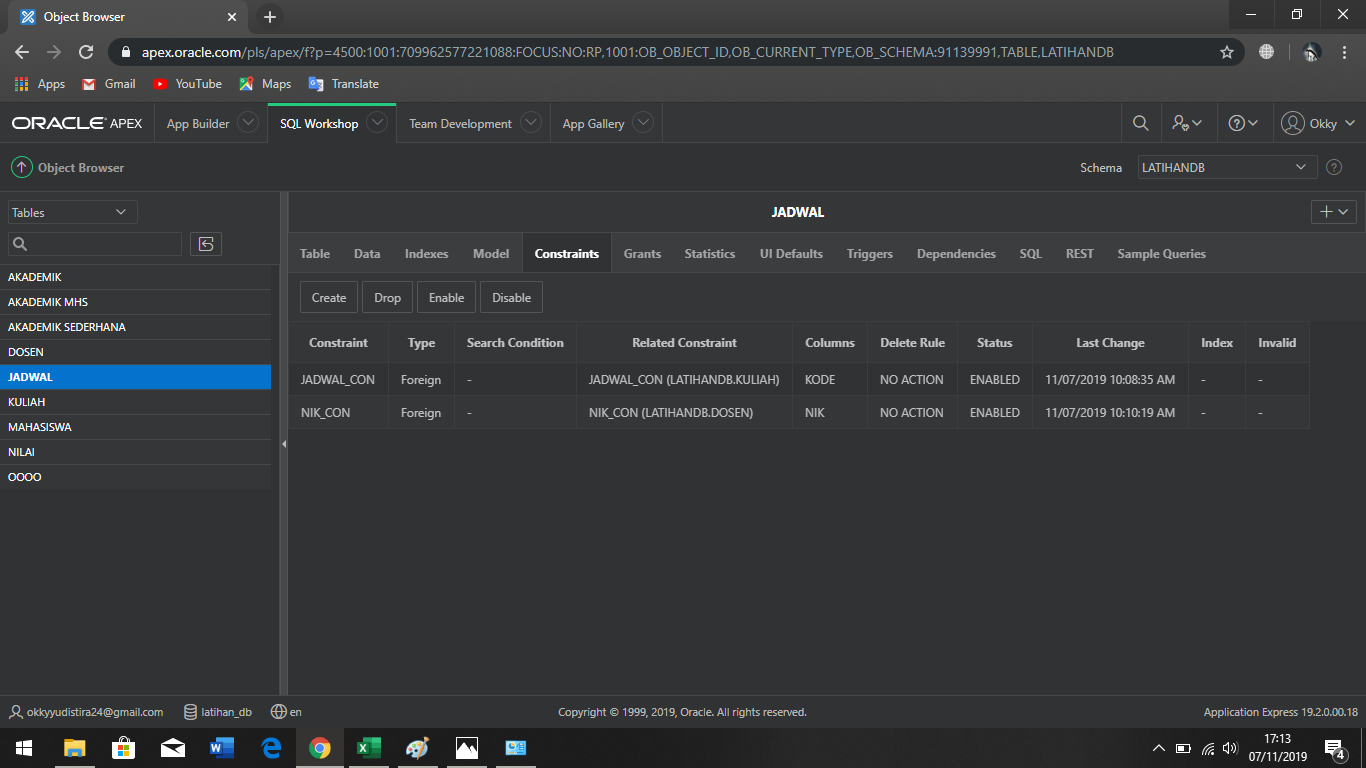
\includegraphics[width=16cm, height=12cm]{pictures/H.png}
        \caption{Contoh FK Pada tabel Jadwal)}
        \label{fig:my_label}
    \end{figure}
    \vspace{2cm}
    
     \section{Menjadikan Aplikasi}
     Setelah Semua table sudah diberi Key dan dianggap sudah baik maka siap dibuat aplikasi. Pilih New Application Untuk membuatnya
     \begin{figure}[!htbp]
        \centering
        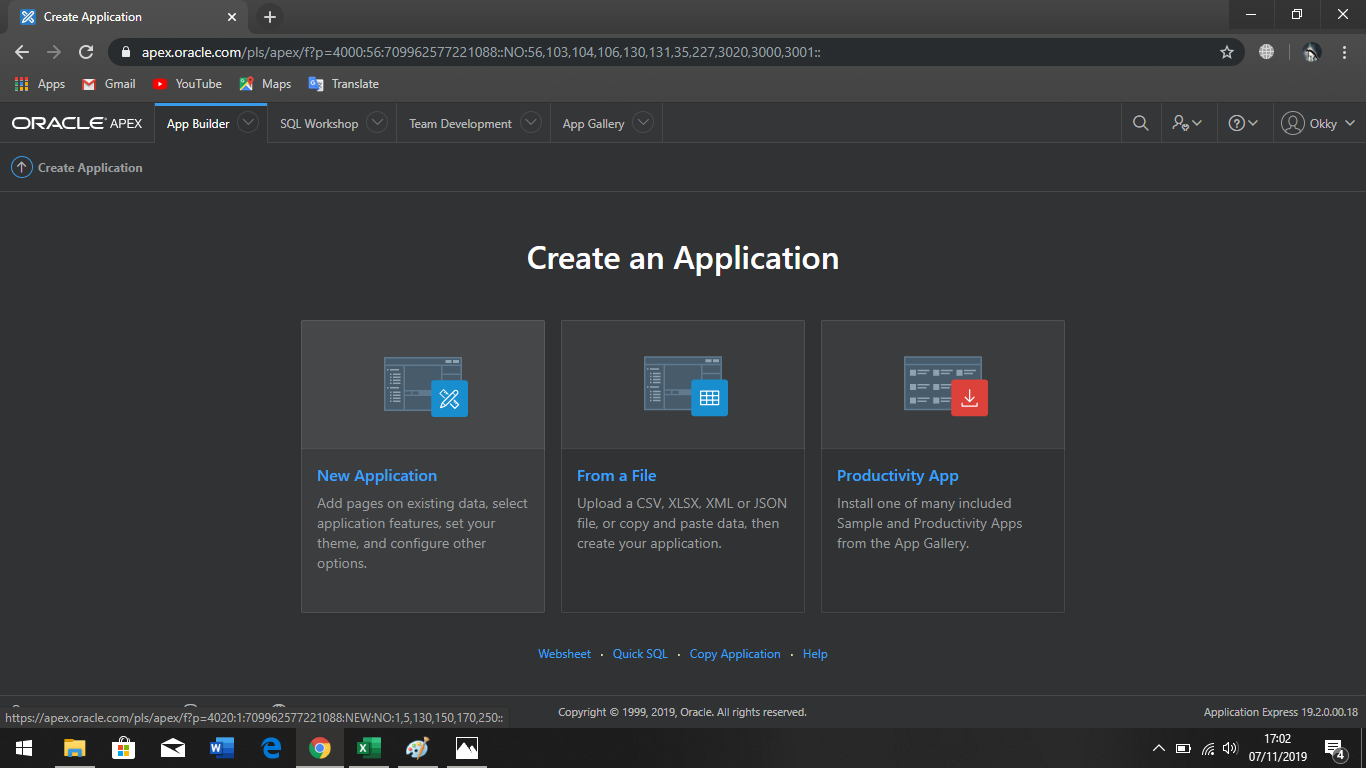
\includegraphics[width=16cm, height=12cm]{pictures/I.png}
        \caption{Contoh Halaman Pada Saat akan membuat suatu aplikasi di apex)}
        \label{fig:my_label}
    \end{figure}
    
      \section{Menambahkan Pages}
     Tambahkan Table tadi untuk di jadikan Page pada aplikasi kita. Nama Aplikasi saya di sini adalah Akademik Sederhan yang berisikan Data yang telah di normalisasi tadi
     \begin{figure}[!htbp]
        \centering
        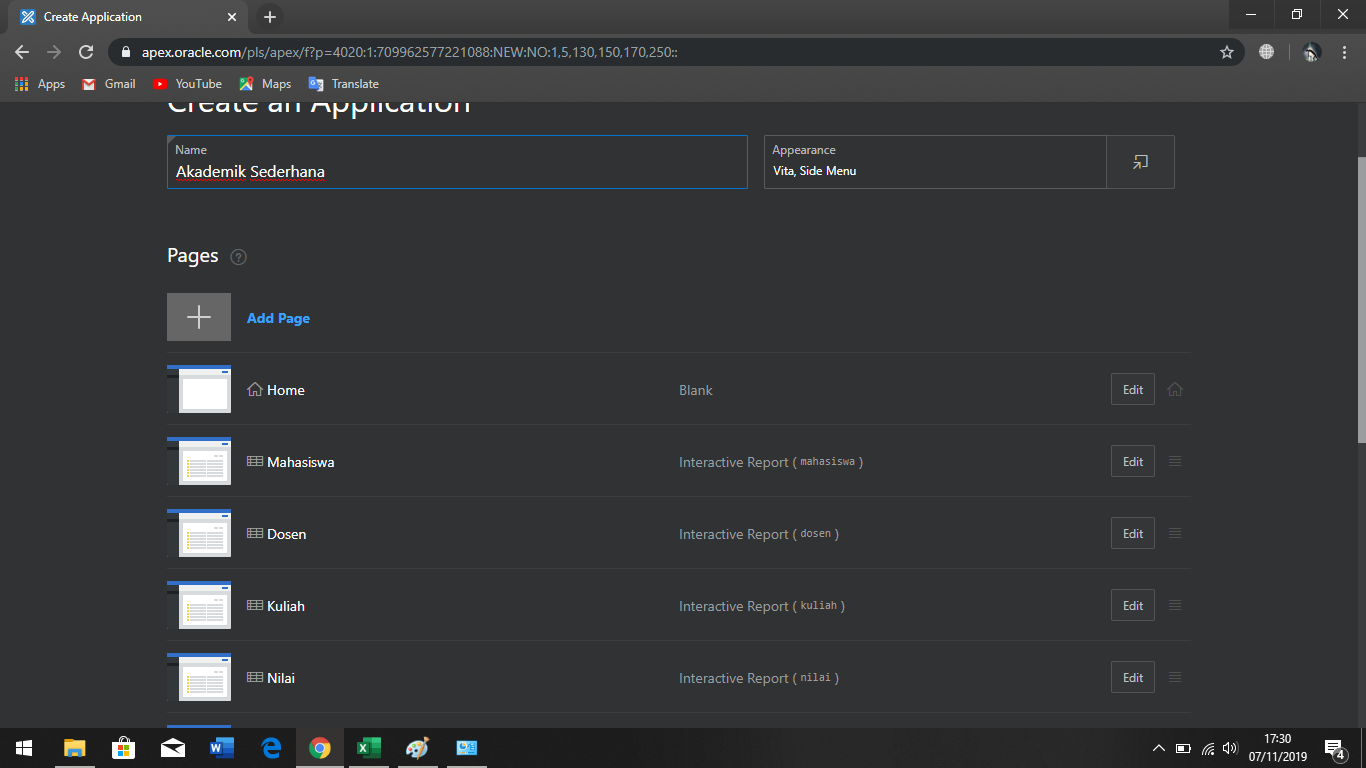
\includegraphics[width=16cm, height=12cm]{pictures/J.png}
        \caption{Contoh Page Yang telah di tambahkan}
        \label{fig:my_label}
    \end{figure}
     \begin{figure}[!htbp]
        \centering
        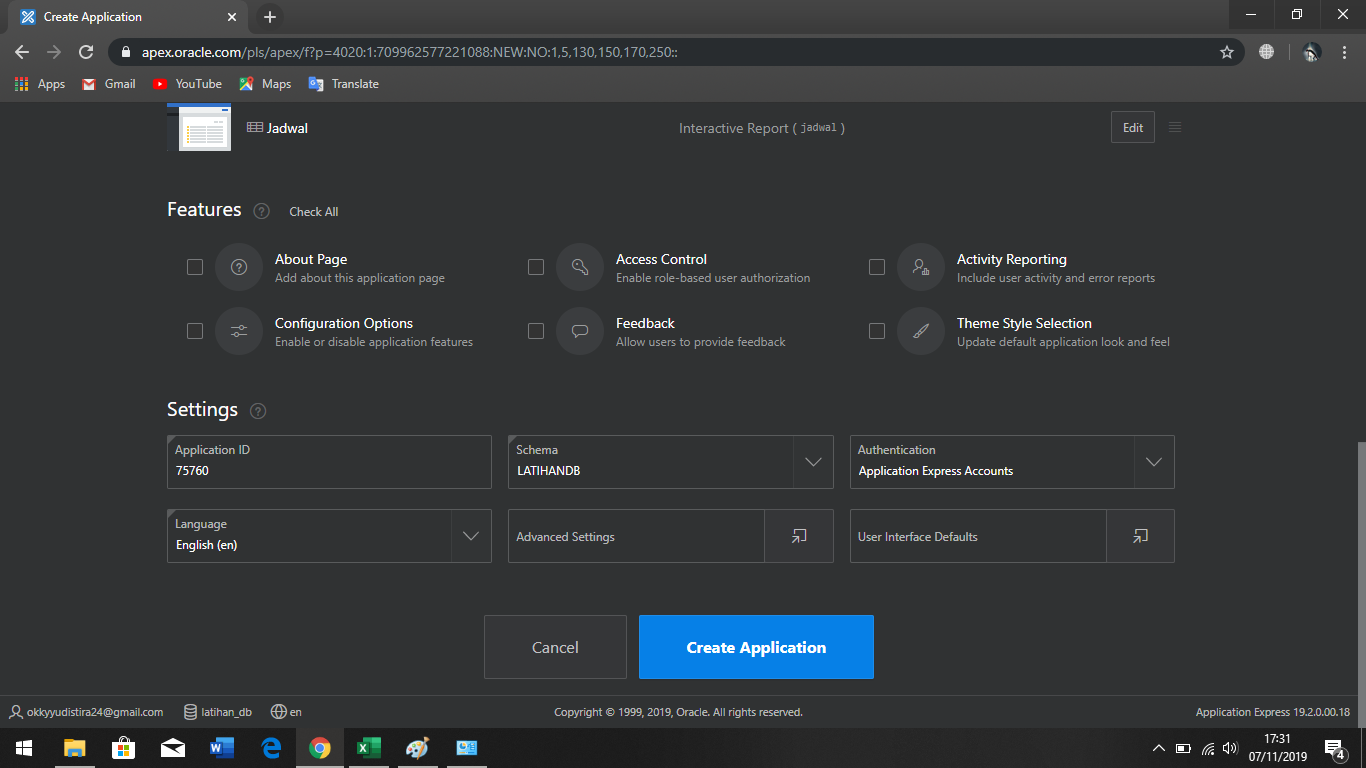
\includegraphics[width=16cm, height=12cm]{pictures/K.png}
        \caption{Create Aplikasi}
        \label{fig:my_label}
    \end{figure}
     \begin{figure}[!htbp]
        \centering
        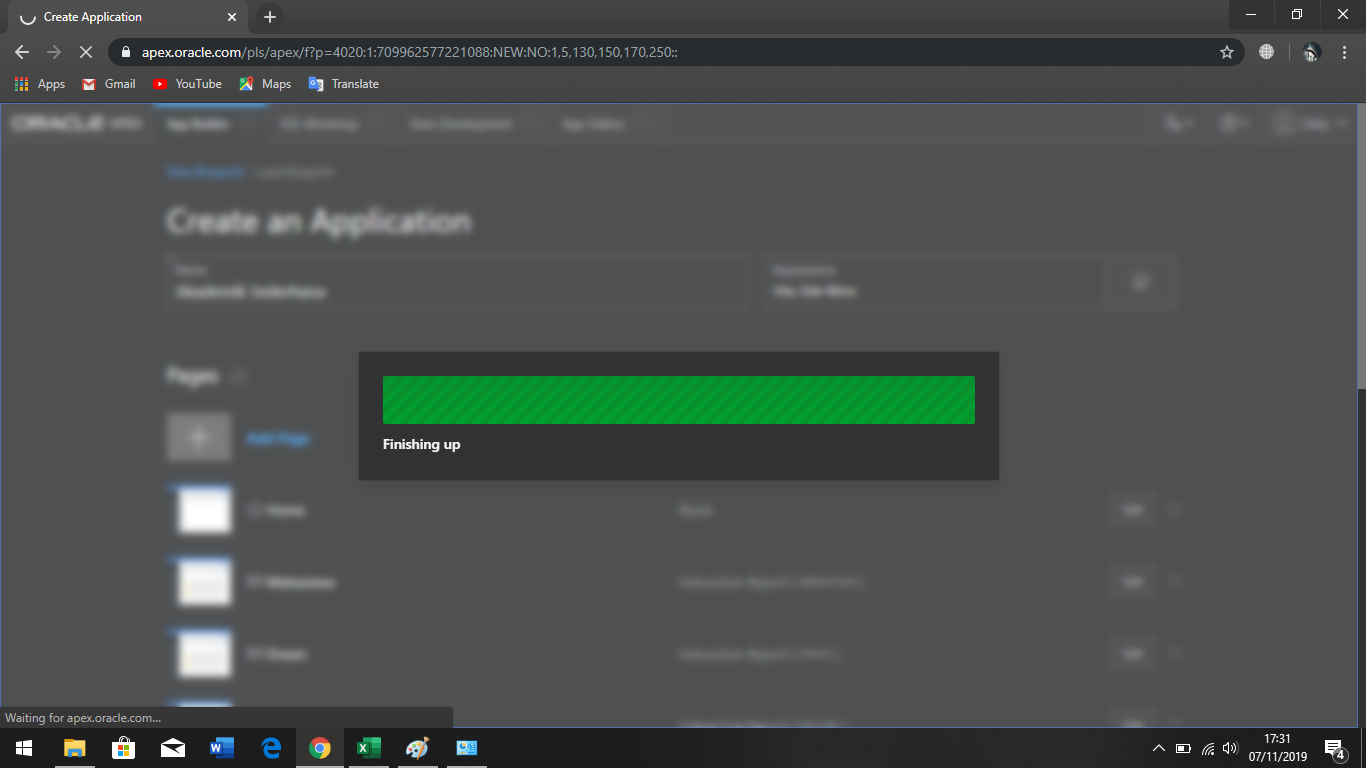
\includegraphics[width=16cm, height=12cm]{pictures/L.png}
        \caption{Loadingn)}
        \label{fig:my_label}
    \end{figure}
    
    \section{Run Application}
    Setelah di bikin Kita masuk ke APP builder Dan siap Run Application
     \begin{figure}[!htbp]
        \centering
        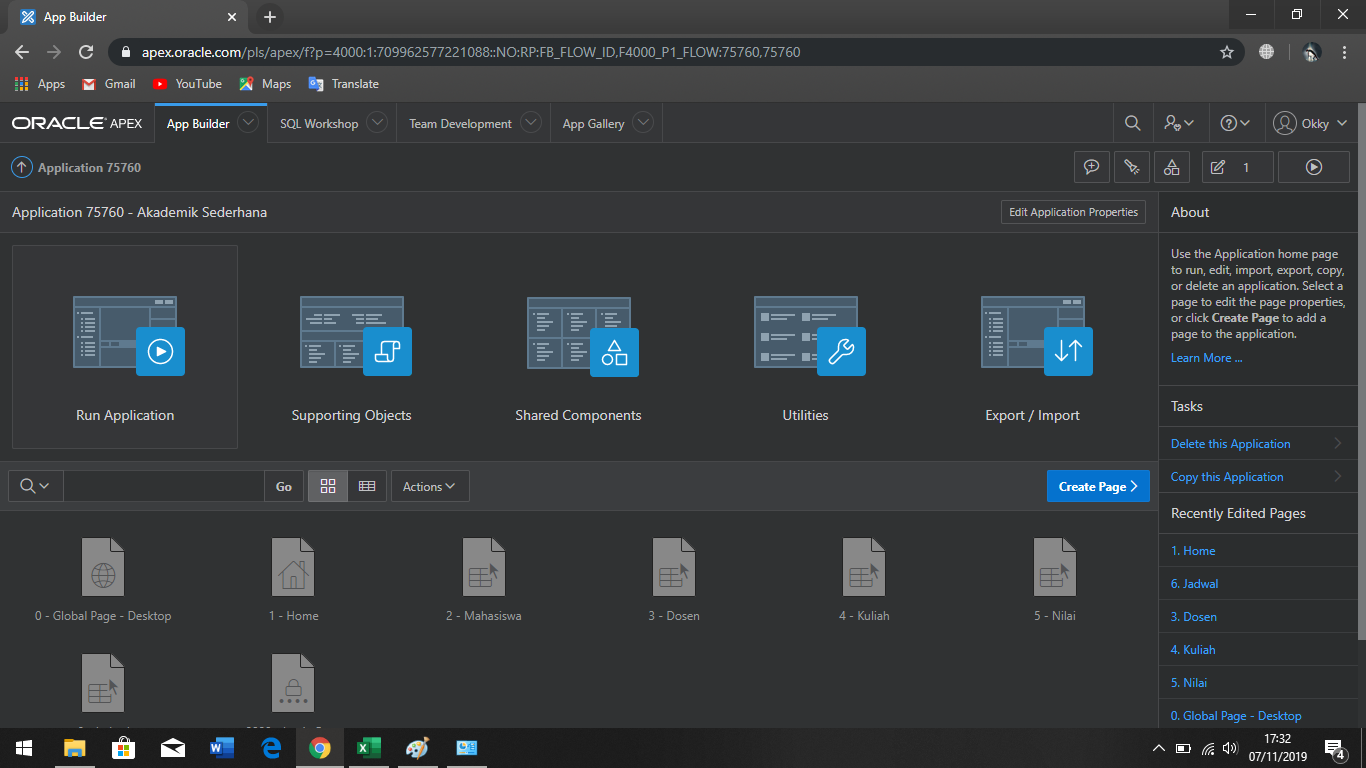
\includegraphics[width=16cm, height=12cm]{pictures/M.png}
        \caption{run application}
        \label{fig:my_label}
    \end{figure}
      \begin{figure}[!htbp]
        \centering
        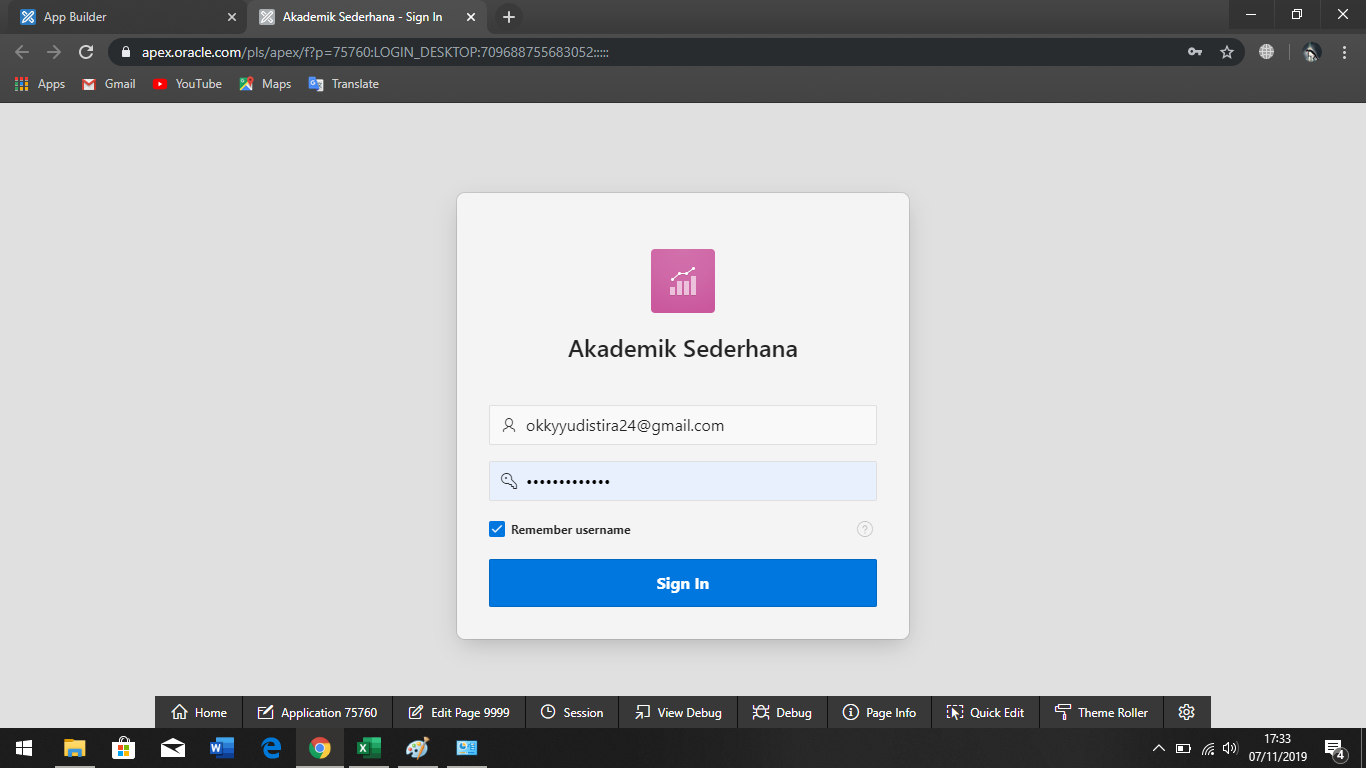
\includegraphics[width=16cm, height=12cm]{pictures/N.png}
        \caption{Masukan Account kalian}
        \label{fig:my_label}
    \end{figure}
    \vspace{3cm}
\section{Last}
Aplikasi sudah jadi dan sesuai dengan table page yang di inputkan. Terimakasih
  \begin{figure}[!htbp]
        \centering
        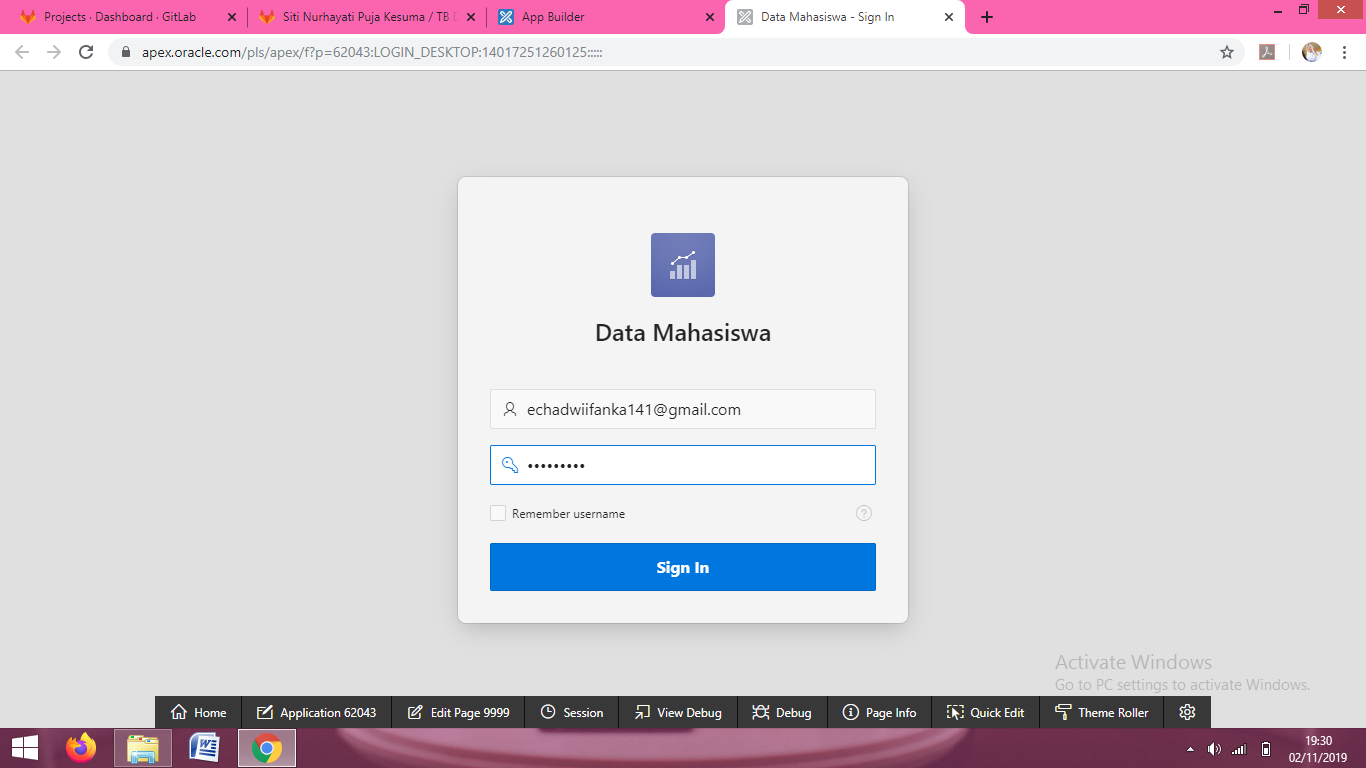
\includegraphics[width=16cm, height=12cm]{pictures/o.png}
        \caption{Menu Aplikasi APEX Online Akademik Sederhana}
        \label{fig:my_label}
    \end{figure}
\end{document}
